
\chapter{Real-time video detection}
\label{chap:rltm}

real time -> 25fps
this is related work
% \section{Optimizing Video Object Detection via a Scale-Time Lattice}
% \section{Use of Detection networks for video processing}

\section{Detection networks}


\subsection{YOLO: You Only Look Once (2016)}
\label{sec:yolo}
Building on the success of neural network detectors from \textit{R-CNN} family. \citeauthor{bib:yolo} \cite{bib:yolo} introduced a new approach to object detection. They unify networks for localization and classification into  a new single network. This network predicts both bounding box positions and class probabilities in a single evaluation. This approach also simplifies the training process, as \textit{YOLO} can be directly trained end-to-end. 

Thanks to straightforward single pass architecture \textit{YOLO} claims to perform at 45 frames per second on \textit{Titan X GPU}. Although it has to sacrifice some precision compared to region proposal methods, it out-performs other real-time systems of its time \cite{bib:overfeat}.


\subsubsection{Detection}
Prediction in \textit{YOLO} work in a grid-based system. It divides the image into \textit{S\x S} grid with each cell responsible for detecting the object centered in that cell.  Each cell produces predictions for \textit{B} bboxes and one set of class confidence predictions. 

Bbox prediction is composed of four positional parameters and confidence score. Center coordinates relate to the grid cell while width and height are represented relative to the whole image. Confidence score reflects IoU with ground-truth box. Class confidence prediction represents the conditional probability of said class, given the presence of the object in that cell. 

Final confidence for each box is the product of both conditional class probabilities and the individual box confidence predictions. We can see the illustration of this process on \cref{fig:yoloDet}.

\begin{figure}
    \centering
    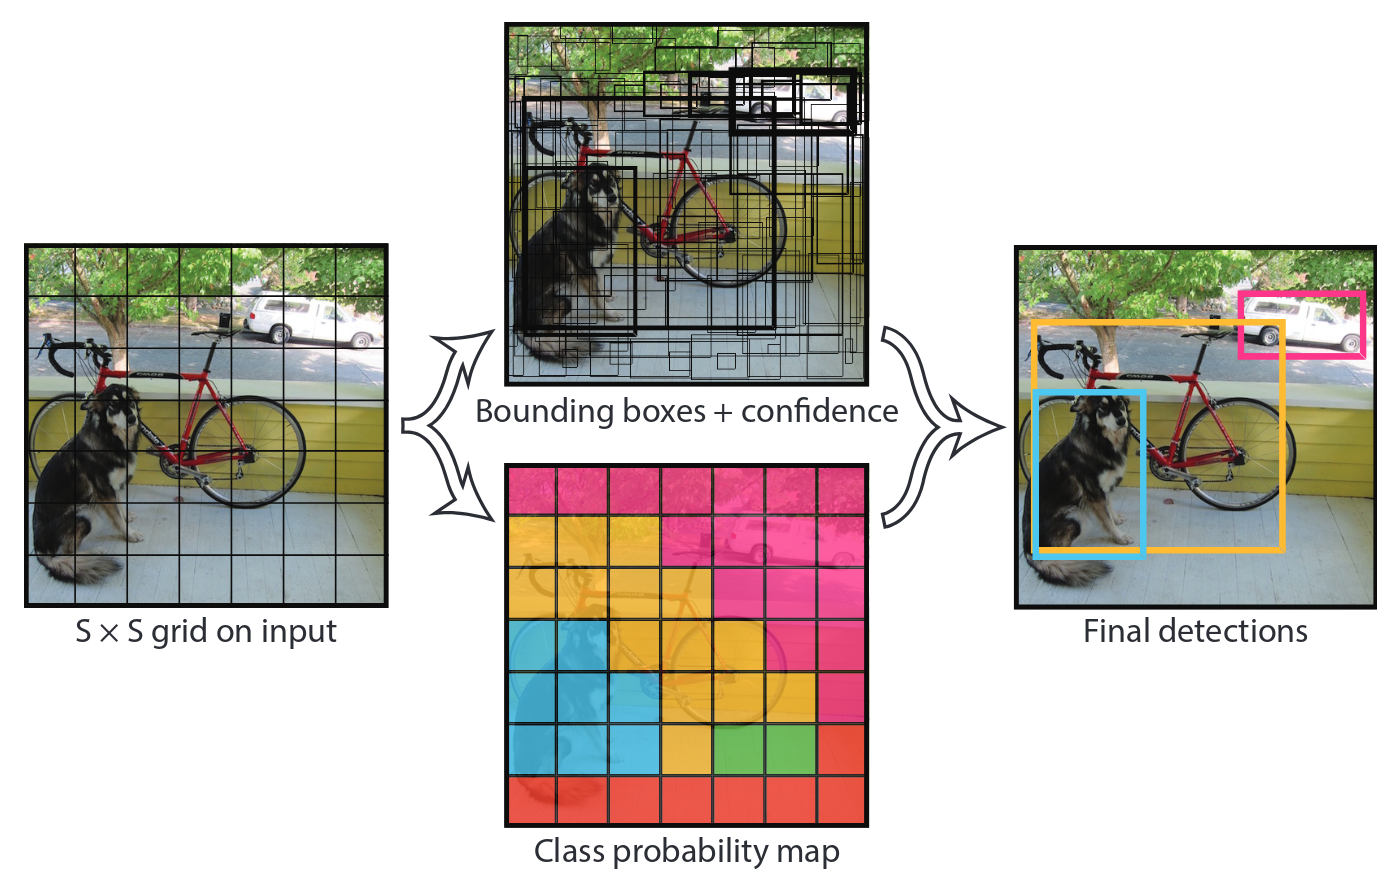
\includegraphics[width=\textwidth]{img/yoloDet}
    \caption{Detection process of \textit{YOLO}. From \cite[fig. 2]{bib:yolo}.}
    \label{fig:yoloDet} 
\end{figure}


\subsubsection{Architecture} 
\textit{YOLO} is designed as a single network that takes the input image and outputs bbox and class predictions. Design of the network is inspired by \textit{Inception} classification network. Although it does not use inception modules, it relies on the 1\x1 reduction layers to speed up 3\x3 convolutions. I\textit{YOLO} t uses 24 convolutional layers followed by two fully connected layers. Full architecture is shown on \cref{fig:yolo}. 

Multiple other versions and modifications are possible. A smaller and faster version is called \textit{Fast YOLO}. It has a similar architecture but uses only 9 convolutional layers. Another possibility to improve \textit{YOLO} is to replace the custom architecture with a more common feature extractor from a classification network. \textit{YOLO} build on top of a \textit{VGG-16} achieves better precision at the cost of half of the frames per second.

\begin{figure}
    \centering
    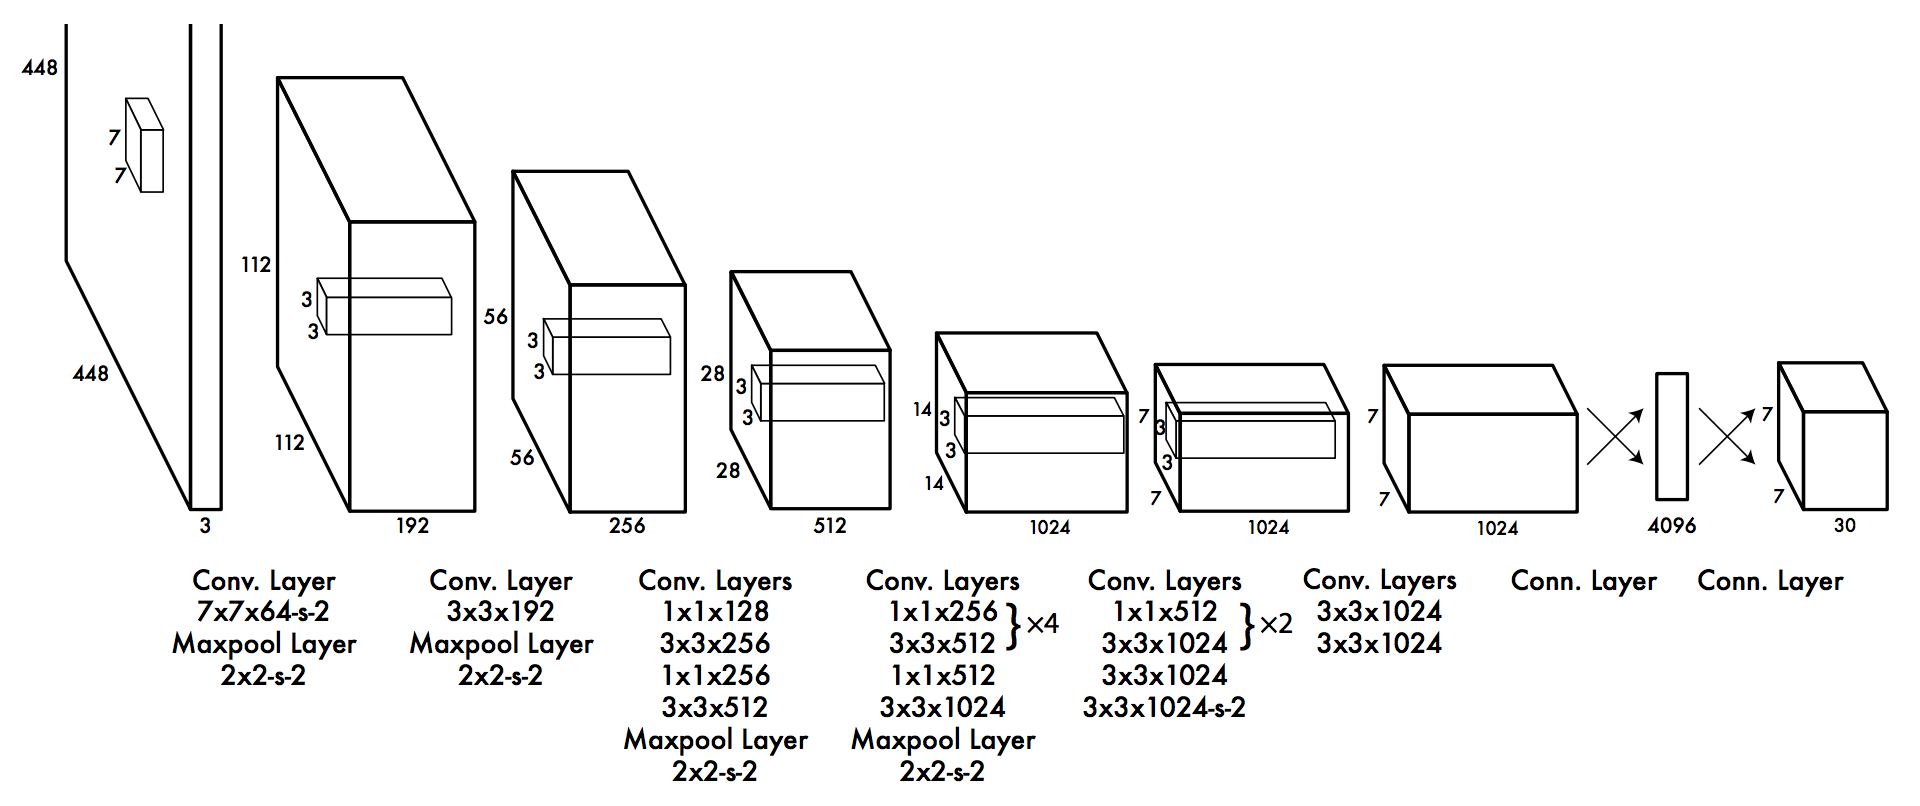
\includegraphics[width=\textwidth]{img/yoylo}
    \caption{\textit{YOLO} architecture for evaluating \textit{PASCAL VOC}. It uses 7 by 7 grid with 2 bboxes per cell. Detecting 20 categories, the output's shape is 7\x7\x30. From \cite[fig. 3]{bib:yolo}.}
    \label{fig:yolo} 
\end{figure}

\subsubsection{Training}
Although the network can be trained end-to-end, it is common for CNN to pre-train on \textit{ImageNet} dataset. This is also the case for \textit{YOLO}. First, convolutional layers are pre-trained on the \textit{ImageNet} dataset, then the detection layers are added and whole network is trained for detection. The model is optimized using sum-squared error between predictions and ground-truths. The loss function is a sum of three parts, classification loss, localization loss, and bbox confidence loss. 

\paragraph{Classification loss}
\begin{align*}
\mathbf{L_{cls}} = \sum_{i=0}^{S^2}\mathbbm{1}_i^{\text{obj}} \sum_{c\in \text{class}} (p_i(c) - \hat{p}_i(c))^2
\end{align*}

\paragraph{Localization loss}
\begin{align*}
\mathbf{L_{loc}} &= \lambda_{\text{coord}} \sum_{i=0}^{S^2} \sum_{j=0}^B \mathbbm{1}_{ij}^{\text{obj}} \left[(x_i - \hat{x}_i)^2 + (y_i - \hat{y}_i)^2\right] \\
 &+  \lambda_{\text{coord}} \sum_{i=0}^{S^2} \sum_{j=0}^B \mathbbm{1}_{ij}^{\text{obj}} \left[(\sqrt{w_i} - \sqrt{\hat{w}_i})^2 + (\sqrt{h_i} - \sqrt{\hat{h}_i)^2}\right]
\end{align*}

\paragraph{Confidence loss}
\begin{align*}
\mathbf{L_{cnf}} &= \sum_{i=0}^{S^2} \sum_{j=0}^B \mathbbm{1}_{ij}^{\text{obj}} (C_i - \hat{C}_i)^2 
+ \lambda_{\text{noobj}} \sum_{i=0}^{S^2} \sum_{j=0}^B \mathbbm{1}_{ij}^{\text{noobj}} (C_i - \hat{C}_i)^2
\end{align*}

\noindent where $\mathbbm{1}^{\text{obj}}_i$ denotes if object appears in cell $i$ and $\mathbbm{1}^{\text{obj}}_{ij}$ denotes that the $j$th bounding box predictor in cell $i$ is responsible for that prediction.

The gradient of cells that do contain the object can be overpowered with the cells that do not.  Therefore, the loss from negative confidence predictions is decreased by $\lambda_{\text{noobj}} = 0.5$. And to emphasize the bbox predictions, localization loss is increased using $\lambda_{\text{coord}} = 5$.In the localization loss, we can see that the center coordinates are handled differently to width and height. The square root of width and height is used to equalize the impact of the absolute value of error in small and large boxes.


\subsubsection{Properties}
A primary virtue of \textit{YOLO} is its speed for real-time applications, and its simple architecture allows for easy training and end-to-end optimization. \textit{YOLO}'s detection layer is provided with context from the whole image which leads to less false detections than in region proposal methods. 

On the other hand, a significant problem with \textit{YOLO}'s grid-based detection system, is a limitation to one class per cell. This limitation results in the inability to detect multiple objects in close proximity, such as people in the crowd. 

\textit{YOLO} also suffers from multiple problems with precise localization. It learns to detect arbitrary shapes, which can be hard to generalize to objects in new and unusual aspect ratios. Also, it predicts the bboxes on the heavily down-sampled image which leads to further imprecision. 


\subsection{SSD: Single Shot MultiBox Detector (2016)}
\label{sec:ssd}
\textit{SSD} is another real-time detector, aiming to outperform \textit{Faster R-CNN} by using a single network with one time evaluation. \citeauthor{bib:ssd} \cite{bib:ssd} presented this model just months after \textit{YOLO}. Both networks are build on similar principles but with multiple key differences. It manages to outperform \textit{Faster R-CNN} and \textit{YOLO} both in speed and precision.

\subsubsection{Detection}
One of the main features of \textit{SSD} is that the detector network is fully convolutional and does not utilize any fully connected layers. Predictions are therefore generated for every position of convolutional window. \textit{SSD} adopts similar concept to \textit{Faster R-CNN's} anchor boxes, this time called \textit{default} or \textit{prior} boxes. For each position of the feature map, multiple prior boxes with different aspect ratios are proposed. By default, 6 boxes are used. Contrary to \textit{YOLO}, both bbox and classification predictions are made for each position and for each prior box.

Bboxes are predicted relative to prior box location which are themselves relative to feature map location. There is no bbox or region confidence value. Instead, \textit{SSD} uses an additional background class in classification predictions. Considering \textit{B} prior boxes and \textit{C} classes, \textit{SSD} generates $m\times n\times B\times (C+5)$ parameters on feature map of m\x n size.

\textit{SSD} detects objects on multiple feature maps with different sizes, to accommodate detection of different sized objects. And allows detectors on each level to focus on predicting smaller range of bbox sizes. For illustration of this process see \cref{fig:ssddet}.

\begin{figure}
    \centering
    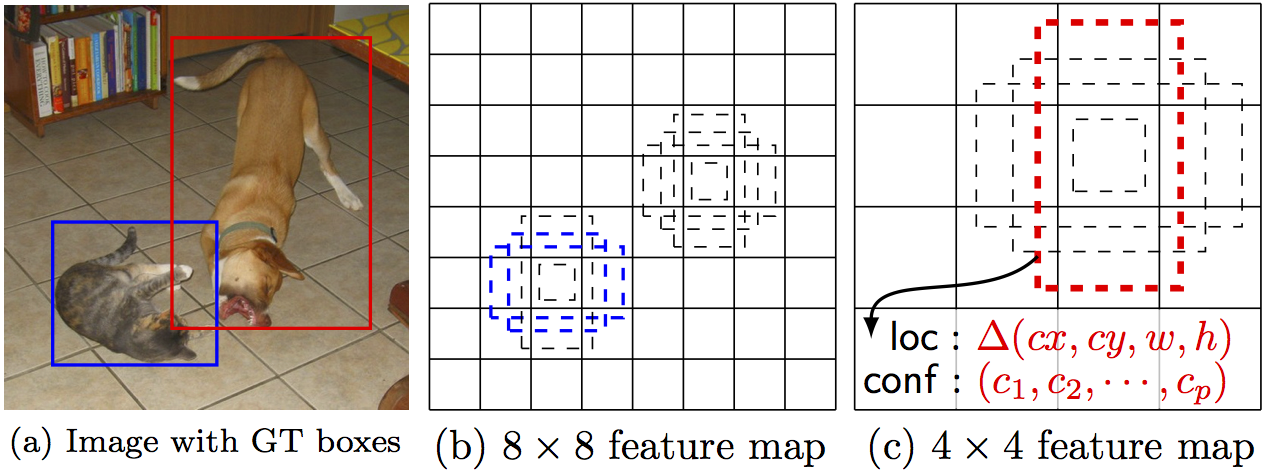
\includegraphics[width=\textwidth]{img/ssddet}
    \caption{SSD detection. (a) Input image with ground-truth boxes. (b) and (c) Predictions based on prior boxes on multiple scales of feature maps.}
    \label{fig:ssddet}
\end{figure}

\subsubsection{Architecture}
The \textit{SSD} architecture can be describe as a set of three modules. A base network, extra convolutional layers and detection layers.

\begin{itemize}
    \item \textbf{Base network}'s task is to take the input image and produce a feature map. To this end, a feature extractor build from classification network is an ideal candidate. \textit{SSDs} base is build from \textit{VGG-16} network with some modifications. First of all, all fully connected layers are removed and replaced with another pair of convolution layers. \textit{Pool5} layer is also changed from 2\x2/2 to 3\x3/1 pooling. Technically, \textit{SSD} does not force any constraints on the base network and the \textit{VGG} can be replaced by any CNN.
    \item \textbf{Extra layers} serve the purpose of providing more feature maps on decreasing scale to the detector. Smaller feature maps aggregate more information to smaller area and allow for detection of larger objects with small convolutional window. On the other hand the information about small objects can be lost. Therefore the use of gradually decreasing series of feature maps. \textit{Extra layers} are implemented as a sequence of convolution layers connected to the end of the \textit{base}.
    \item \textbf{Detection layers} are the final layers of the network. There is a pair of classification and localization convolutions for each feature map. Considering \textit{SSD300}, where 300 stands for the width and height of input image. Detection is performed on 6 feature maps of sizes [38, 19, 10, 5, 3, 1], using [4, 6, 6, 6, 4, 4] prior boxes respectively, producing 8732 predictions per class. First two of those feature maps are pulled from the \textit{VGG} network and the rest is provided by the \textit{extra layers}. All detection layers are implemented using 3\x3 convolutions with appropriate number of filters, as seen on \cref{fig:VGGSSD}.
\end{itemize}

\begin{figure}
    \VGGSSD
    \caption{SSD architecture based on modified \textit{VGG-16} network. \textit{VGGs} three fully connected layers are replaced with two new convolutional layers and \textit{Pool5} layer is changed from 2\x2/2 to 3\x3/1 pooling. Detection on the first and last two feature maps uses 4 prior boxes, while the rest uses 6 boxes. See more details on \textit{VGG} in \cref{sec:VGG}.}
    \label{fig:VGGSSD}
\end{figure}


\subsubsection{Training}
\todo{matching}

Similarly to \textit{YOLO}, \textit{SSD} also pre-trains the \textit{base network} on \textit{ImageNet} dataset before removing the classification layers and replacing them with \textit{extra} and \textit{detection} layers. The model is than trained for detection end-to-end. \textit{SSD} utilizes \textit{smooth L1} loss for localization and \textit{cross-entropy} loss for classification. The final loss is the sum of those two components.

\paragraph{Localization loss}

\begin{align*}
\mathbf{L_{\text{loc}}}(x,l,g) = \sum_{i\in Pos}^N \sum_{m\in(cx, cy, w, h)} &x_{ij}^k\text{smooth}_{L1}(l_i^m-\hat{g}_j^m) \\
\hat{g}_j^{cx} = (g_j^{cx} - d_i^{cx}) / d_i^{w} \qquad& \hat{g}_j^{cy} = (g_j^{cy} - d_i^{cy}) / d_i^{h} \\
\hat{g}_j^{w} = log(\frac{g_j^{w}}{d_i^w}) \qquad& \hat{g}_j^{h} = log(\frac{g_j^{h}}{d_i^h})
\end{align*}
where the ground-truths are encoded in respect to their matching prior boxes


\paragraph{Classification loss}
\begin{align*}
\mathbf{L_{\text{cls}}}(x,c) = -\sum_{i\in Pos}^N x_{ij}^p log(\hat{c}_i^p) - \sum_{i \in Neg} log(\hat{c}_i^0) \quad\text{where} \quad\hat{c}_i^p = \frac{exp(c_i^p)}{\sum_p exp(c_i^p)}
\end{align*}



\subsubsection{Properties}


\subsection{200fps}
\todo{ https://arxiv.org/pdf/1805.06361.pdf}

\section{video smthing}
\subsection{Optimizing Video Object Detection via a Scale-Time Lattice}
